\documentclass[11pt]{article}

\usepackage[margin=1in]{geometry}
\usepackage{xcolor}
\usepackage{amsmath}
\usepackage{fancyhdr}
\usepackage{graphicx}
\usepackage{enumitem}
\usepackage{pgfplots}
\usepackage{booktabs}
\usepackage{float}

\pgfplotsset{compat=1.18}

% Define colors
\definecolor{sectioncolor}{RGB}{0,51,102}

% Configure headers and footers
\pagestyle{fancy}
\fancyhf{}
\fancyhead[L]{\textit{COMP 6231 Assignment 3}}
\fancyhead[R]{\textit{Fall 2025}}
\fancyfoot[C]{\thepage}
\renewcommand{\headrulewidth}{0.4pt}
\renewcommand{\footrulewidth}{0.4pt}

% Section formatting
\usepackage{titlesec}
\titleformat{\section}
{\color{sectioncolor}\normalfont\Large\bfseries}
{\color{sectioncolor}\thesection}{1em}{}[\color{sectioncolor}\titlerule]

\titleformat{\subsection}
{\color{sectioncolor}\normalfont\large\bfseries}
{\color{sectioncolor}\thesubsection}{1em}{}

\title{\textbf{\Large COMP 6231 Assignment 3}\\[0.5em]
\textbf{\large Task 2: MPI Performance Analysis}}
\author{
    \small
    \begin{tabular}{c}
        Qiang Xue (40300671) \quad Yicheng Cai (26396283) \quad Yikai Chen (40302669)\\[0.3em]
        Yifan Wu (40153584) \quad Alexander Sutherland (40321783)
    \end{tabular}
}

\begin{document}
\maketitle
\thispagestyle{fancy}


\section{Overview}

The MPI cluster consists of 11 containers (1 master + 10 workers) distributed across four physical computers. Four analysis scripts (q1\_t3.py through q4\_t3.py) were executed with varying container counts (4-10) using the Books\_rating.csv dataset. Execution times were measured for each configuration to evaluate scalability.

\section{Execution Time Results}

\begin{table}[H]
\centering
\begin{tabular}{ccccc}
\toprule
\textbf{Worker Containers} & \textbf{Q1 (s)} & \textbf{Q2 (s)} & \textbf{Q3 (s)} & \textbf{Q4 (s)} \\
\midrule
4 & 5.697 & 6.530 & 8.673 & 6.553 \\
5 & 9.661 & 9.304 & 13.038 & 10.614 \\
6 & 12.017 & 12.348 & 12.451 & 12.431 \\
7 & 10.961 & 10.769 & 10.697 & 11.279 \\
8 & 15.865 & 13.819 & 14.295 & 13.319 \\
9 & 14.445 & 12.109 & 12.676 & 13.091 \\
10 & 15.424 & 13.615 & 13.621 & 12.144 \\
\bottomrule
\end{tabular}
\caption{Execution times for all four analysis scripts}
\label{tab:results}
\end{table}

\section{Performance Analysis}

\begin{figure}[H]
\centering
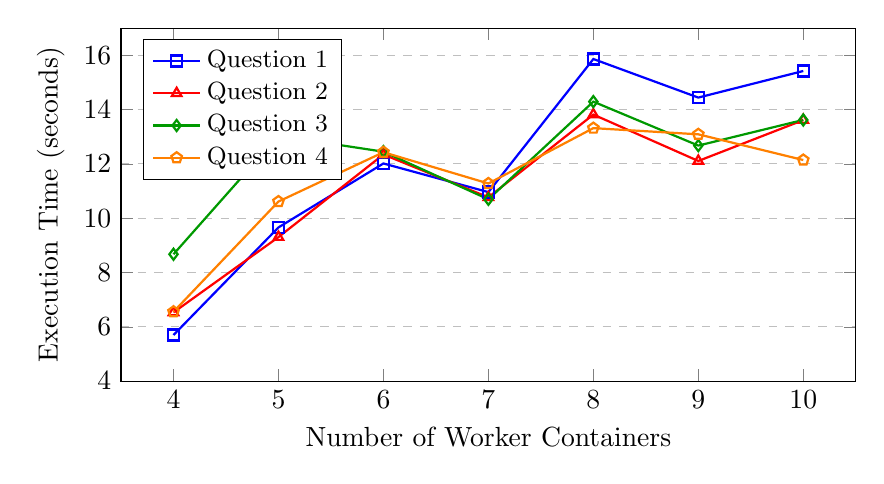
\begin{tikzpicture}
\begin{axis}[
    width=0.9\textwidth,
    height=0.5\textwidth,
    xlabel={Number of Worker Containers},
    ylabel={Execution Time (seconds)},
    xmin=3.5, xmax=10.5,
    ymin=4, ymax=17,
    xtick={4,5,6,7,8,9,10},
    ytick={4,6,8,10,12,14,16},
    legend pos=north west,
    ymajorgrids=true,
    grid style=dashed,
    legend style={font=\small},
]

\addplot[color=blue, mark=square, thick] coordinates {
    (4,5.697)(5,9.661)(6,12.017)(7,10.961)(8,15.865)(9,14.445)(10,15.424)
};
\addlegendentry{Question 1}
    
\addplot[color=red, mark=triangle, thick] coordinates {
    (4,6.530)(5,9.304)(6,12.348)(7,10.769)(8,13.819)(9,12.109)(10,13.615)
};
\addlegendentry{Question 2}
    
\addplot[color=green!60!black, mark=diamond, thick] coordinates {
    (4,8.673)(5,13.038)(6,12.451)(7,10.697)(8,14.295)(9,12.676)(10,13.621)
};
\addlegendentry{Question 3}

\addplot[color=orange, mark=pentagon, thick] coordinates {
    (4,6.553)(5,10.614)(6,12.431)(7,11.279)(8,13.319)(9,13.091)(10,12.144)
};
\addlegendentry{Question 4}

\end{axis}
\end{tikzpicture}
\caption{Execution time vs. number of containers}
\label{fig:performance}
\end{figure}

\subsection{Key Observations}

\begin{itemize}[leftmargin=*,itemsep=4pt]
    \item \textbf{Optimal Performance at 4 Containers:} All four scripts achieved best performance with 4 containers (5.7-8.7 seconds). This configuration places exactly one worker container on each of the four physical computers, eliminating resource contention within individual machines and maximizing network bandwidth utilization per node.
    
    \item \textbf{Performance Degradation Beyond 4 Containers:} Increasing containers beyond 4 forces multiple containers to share resources on the same physical machines, causing CPU, memory, and network bandwidth contention. At 8 containers, execution times increased by 65-178\% compared to the 4-container baseline due to intra-machine resource competition and increased inter-container communication overhead.
    
    \item \textbf{Resource Contention:} With more than 4 containers, multiple workers on the same physical machine compete for shared resources (CPU cores, memory bandwidth, network interface). This contention, combined with increased MPI communication overhead (scatter, gather, synchronization), severely degrades performance.
    
    \item \textbf{Question 3 Complexity:} Q3 consistently shows highest execution times across all configurations, suggesting it involves more communication-intensive operations that are particularly sensitive to resource contention and network overhead.
\end{itemize}

\section{Conclusions and Lessons Learned}

\subsection{Key Findings}

\begin{itemize}[leftmargin=*,itemsep=4pt]
    \item \textbf{Optimal Configuration:} 4 containers (one per physical computer) provide the best performance by eliminating intra-machine resource contention while maintaining efficient inter-machine parallelization.
    
    \item \textbf{Physical Distribution Impact:} Performance degrades when multiple containers share the same physical machine due to CPU, memory, and network bandwidth competition. The 4-container configuration avoids this contention entirely.
    
    \item \textbf{Scalability Limitation:} Beyond 4 containers, the system suffers from both intra-machine resource contention and increased MPI communication overhead, causing performance to degrade rather than improve.
    
    \item \textbf{Communication vs. Resource Bottleneck:} The primary bottleneck is not just MPI communication overhead, but the combination of resource contention on physical machines hosting multiple containers and the resulting network congestion.
\end{itemize}

\subsection{Lessons Learned}

\begin{itemize}[leftmargin=*,itemsep=4pt]
    \item \textbf{Container Distribution:} Always distribute containers to maximize one-container-per-physical-machine deployment. For this 4-machine cluster, use exactly 4 containers for optimal performance.
    
    \item \textbf{Scaling Strategy:} To achieve better scalability beyond 4 containers, add more physical machines rather than deploying multiple containers on existing machines. Each additional physical computer can host one more container without resource contention.
    
    \item \textbf{Resource Isolation:} If multiple containers per machine are necessary, ensure adequate CPU cores, memory, and dedicated network bandwidth to minimize contention. Consider using Docker resource limits and CPU pinning.

\end{itemize}

\end{document}